\documentclass[pdflatex,Numbered]{sn-jnl}

\usepackage[T1]{fontenc}
\usepackage[utf8]{inputenc}
\usepackage{amsmath,amssymb}
\usepackage{booktabs}
\usepackage{graphicx}
\usepackage{microtype}
\usepackage{xcolor}
\usepackage{setspace}
\usepackage{lineno}
\usepackage[numbers,sort&compress]{natbib}
\usepackage{tikz}
\usepackage{hyperref}
\usetikzlibrary{arrows.meta,positioning,shadows.blur,fit}

\graphicspath{{./figures/}}
\geometry{a4paper,left=1.8cm,right=1.8cm,top=1.8cm,bottom=1.8cm}
\setlength{\textfloatsep}{10pt plus 2pt minus 2pt}
\setlength{\floatsep}{10pt plus 2pt minus 2pt}
\setlength{\intextsep}{10pt plus 2pt minus 2pt}
\setlength{\dbltextfloatsep}{10pt plus 2pt minus 2pt}
\setlength{\dblfloatsep}{10pt plus 2pt minus 2pt}

\title{A regional traffic simulation from mobile-phone, detector and GPS data: what each source adds, tested on independent observations}

\author*[1]{\fnm{Federico} \sur{Bellisardi}}\email{fbellisardi@ifisc.uib-csic.es}
\author[2]{\fnm{Chiara} \sur{Mizzi}}
\author[2]{\fnm{Alessandro} \sur{Fabbri}}
\author[3,4]{\fnm{Armando} \sur{Bazzani}}

\affil*[1]{\orgdiv{Instituto de F\'{\i}sica Interdisciplinar y Sistemas Complejos IFISC}, \orgname{CSIC-UIB}, \street{Campus UIB}, \postcode{07122}, \city{Palma de Mallorca}, \country{Spain}}
\affil[2]{\orgname{Mindicity}, \country{Italy}}
\affil[3]{\orgdiv{Department of Physics and Astronomy ``Augusto Righi''}, \orgname{University of Bologna}, \street{Viale Carlo Berti Pichat 6/2}, \postcode{40127}, \city{Bologna}, \country{Italy}}
\affil[4]{\orgname{INFN, Sezione di Bologna}, \street{Viale Carlo Berti Pichat 6/2}, \postcode{40127}, \city{Bologna}, \country{Italy}}

\abstract{Managing a regional road network requires knowing how much traffic each road carries through the day, yet no single data source shows this. Mobile phones reveal where people travel but not which roads they take, loop detectors count vehicles at only a few points, and GPS-equipped vehicles are a small and uneven sample of traffic. Models that combine these sources are often judged on the data used to build them, so it is hard to tell what each source really adds. We built an agent-based simulation of road traffic in Emilia-Romagna, Italy, in which phone records supply the trips, detector counts set their number and correct flows locally, and GPS traces from one province guide route choice. We assessed each step on data that did not set its values and against simple predictors that use no simulation. The model reproduces the overall volume, the ranking of roads and the daily timing of traffic in two seasons, with scaling by province removing most of the regional bias and GPS-informed routing improving the ranking of roads. The origin--destination relations used by the model, by contrast, have no clear effect of their own on road volumes, and an average detector profile gives better timing than the simulation. At single roads the model falls well short of the usual accuracy criterion and has not been shown to beat predictors based on road class and other detectors; the remaining error is stable over time and specific to each road.}

\keywords{traffic reconstruction, mobile-phone demand, inductive loop detectors, GPS probes, route choice, agent-based simulation}

\begin{document}
\maketitle
\singlespacing % \doublespacing for a review copy
\linenumbers

\section{Introduction}
\label{sec:intro}

Knowing how much traffic each road of a region carries, hour by hour, is basic information for transport planning \cite{toole2015}, for understanding congestion \cite{colak2016} and for assessing emissions \cite{grujic2022}. No single data source provides it. Mobile phones show where people travel but not which roads they take, and phone samples carry biases of their own \cite{gonzalez2008,calabrese2011,wesolowski2013}. Loop detectors count every vehicle, but only at a few points, and their placement limits what can be inferred about the rest of the network \cite{yang1998,castillo2008,gentili2012,castillo2015}. GPS-equipped vehicles cover many roads, but they are a small sample of traffic, and the chance that a vehicle is sampled varies between roads and hours \cite{herrera2010,jenelius2013,patire2015}. A regional model therefore has to combine these sources \cite{elfaouzi2011,zheng2014,chen2016,anda2017}, which raises a simple question: what does each of them actually contribute?

Each source has a long history of its own. Phone and GPS data have revealed statistical regularities in individual mobility \cite{bazzani2010,gallotti2016,mizzi2018,mizzi2022,mizzi2023,bellisardi2025}. Phone records have also been used to estimate origin--destination (OD) matrices \cite{iqbal2014,alexander2015}, and these matrices have been routed on road networks with assignment models \cite{wardrop1952} to study road usage and congestion \cite{wang2012,toole2015,colak2016}. Detector counts have long been used to estimate OD matrices \cite{cascetta1984,yang1992,antoniou2016} and to calibrate agent-based simulations \cite{flotterod2011}. Probes and fixed sensors feed methods that estimate the state of traffic, mostly on motorways and urban corridors \cite{wang2005,work2010,bachmann2013,seo2015,nantes2016,seo2017}.

More recent work brings the sources together. Telecom data have been fused with vehicle flows to predict traffic where no camera is available \cite{lin2024}, traffic states have been estimated at locations without sensors \cite{lei2024}, and sparse fixed sensors have been scaled up to describe whole urban networks \cite{maiti2025}. Closer to our work, agent-based simulations now take their demand from phone data: in Barcelona, activity diaries built from phone records feed a MATSim model \cite{bassolas2019}, in Novi Sad telecom data are combined with population and GIS data and traffic is calibrated and validated with vehicle counters \cite{grujic2022}, and aggregated phone data have been used to generate a model of Brussels \cite{li2024}. A recent review of more than 60 such case studies shows how common this kind of data-driven, city-wide simulation has become \cite{bochenina2025}. Combining the sources is therefore no longer new, and doing so does not in itself show what each of them adds.

Three things make that contribution hard to see. First, independent observations are scarce. Simulations need validation against data not used for calibration \cite{toledo2004,hollander2008}, yet demand is often rescaled to match the counts, and agreement at those same counts is then reported. The closest studies show how limited the options can be: \c{C}olak et al.\ report that no single validation source existed for their cities \cite{colak2016}, Toole et al.\ compare their estimates with travel surveys \cite{toole2015}, and Bassolas et al.\ keep traffic counts out of the calibration but have them only at some main entrances of the city \cite{bassolas2019}. Second, the sources are usually assessed together, so the result shows whether the complete model works, not which source made it work, even though uncertainty in demand propagates through every modelling stage \cite{zhao2002,rasouli2012}. Third, the model needs a benchmark. Simple historical profiles are strong predictors of the daily pattern of traffic \cite{lippi2013,vlahogianni2014}, so good timing means little unless a model is shown to do better than they do.

In this paper we address these three points for a whole region, with an hourly simulation of the regional road network of Emilia-Romagna, Italy. We do not claim a more accurate model than earlier ones, and no common benchmark would allow such a claim. What our analysis adds is a measure of what each source contributes. We give each source one job in the model and check that job with data that played no part in it (Table~\ref{tab:roles}). Half of the detectors scale the demand, with one factor per day type and one per province, while route choice uses GPS measured in one province and transferred to the rest of the region by road class. We assess timing on all GPS-matched roads, volumes at independent detectors in two seasons and a local correction by withholding each detector in turn, always against predictors that use no simulation. We also test what changes when the OD relations are removed. Section~\ref{sec:data} describes the data and Section~\ref{sec:methods} the model and the tests. Section~\ref{sec:results} follows the model as it is built, from the level of traffic to its timing, the ranking of roads, the correction and the OD relations, and ends with what each source adds. Section~\ref{sec:discussion} discusses what this means and where the model stops.

\begin{table}[htbp]
\centering
\caption{Role of each data source. Each step is assessed with data that did not enter it; the depth of the correction is the one exception, explained in note~$a$.}
\label{tab:roles}
\begin{tabular}{@{}p{3.6cm}p{5.4cm}p{6.0cm}@{}}
\toprule
Data & Enters the model in & Used to validate \\
\midrule
Mobile-phone OD (Jan--Feb 2020) & where and when trips occur & -- \\
GPS traces, Forl\`i--Cesena & route choice (class speeds and usage) & -- \\
GPS link counts, two campaigns & -- & hourly profiles on all matched links \\
Detectors, half of February 2020 & demand scale $k$, province factors, trip radius, departure shift, depth$^{a}$ & -- \\
Detectors, other half of February 2020 & local correction; adoption of province factors$^{b}$ & volume level and ranking (2020) \\
Detectors, June--July 2021 & local correction; adoption of province factors$^{b}$ & volume level and ranking, later season \\
Detector withheld from correction & -- & leave-one-detector-out test \\
\bottomrule
\end{tabular}
\par\vspace{2pt}{\footnotesize $^{a}$The depth of the correction was selected by cross-validation over all detectors of 2020; 2021 is independent of it. $^{b}$These detectors decided once whether the factors, set on the calibration half, were kept; they set no value.}
\end{table}

\section{Data}
\label{sec:data}

The road network comes from OpenStreetMap \cite{osm,boeing2017}, whose road coverage has been estimated to exceed 95\% in most European countries \cite{barrington2017}. It has 3,925 links and 2,548 nodes, with their length, direction and turn restrictions, and each link carries an OpenStreetMap road class (Fig.~\ref{fig:inputs}a). The network marks 122 links (151~km of 11,734~km) as closed, and simulated vehicles cannot use them. We kept these flags as they are, even though two detectors lie on closed links. One of the two, detector 153, records about 11,000 vehicles per day, so on that road either the closure or the placement of the detector must be wrong.

For the demand, the operator TIM provided hourly activity between municipalities for 13 January--23 February 2020, which we averaged separately for each day of the week. The model keeps the relations among the 50 most active municipalities and between them and the provinces of neighbouring regions. When one end of a trip, or both, lies outside this set, the model draws the missing end at random. We left out trips within a single municipality (about 1.2 million agents on a Monday), because adding them did not reduce the spread of the errors on the calibration detectors (Supplementary Section~S2).

Only part of the recorded activity therefore enters the model as a relation. On a Monday, 20\% of the activity between municipalities keeps its relation, 30\% has no identified destination and about 50\% has a recorded relation that the model does not use; trips within a municipality are a further 44\% of the table. The result is 2.01 million agents on a Monday, of which 20\% have a known origin and destination and 80\% have at least one random end (Fig.~\ref{fig:demand}; Supplementary Section~S1). Because the same averages serve every simulated day, eight simulations cover the fifteen days of the two campaigns, and the 2021 days use demand measured in early 2020. The hour labels in the tables refer to local time at the start of the hour (Supplementary Section~S7).

\begin{figure*}[htbp]
\centering
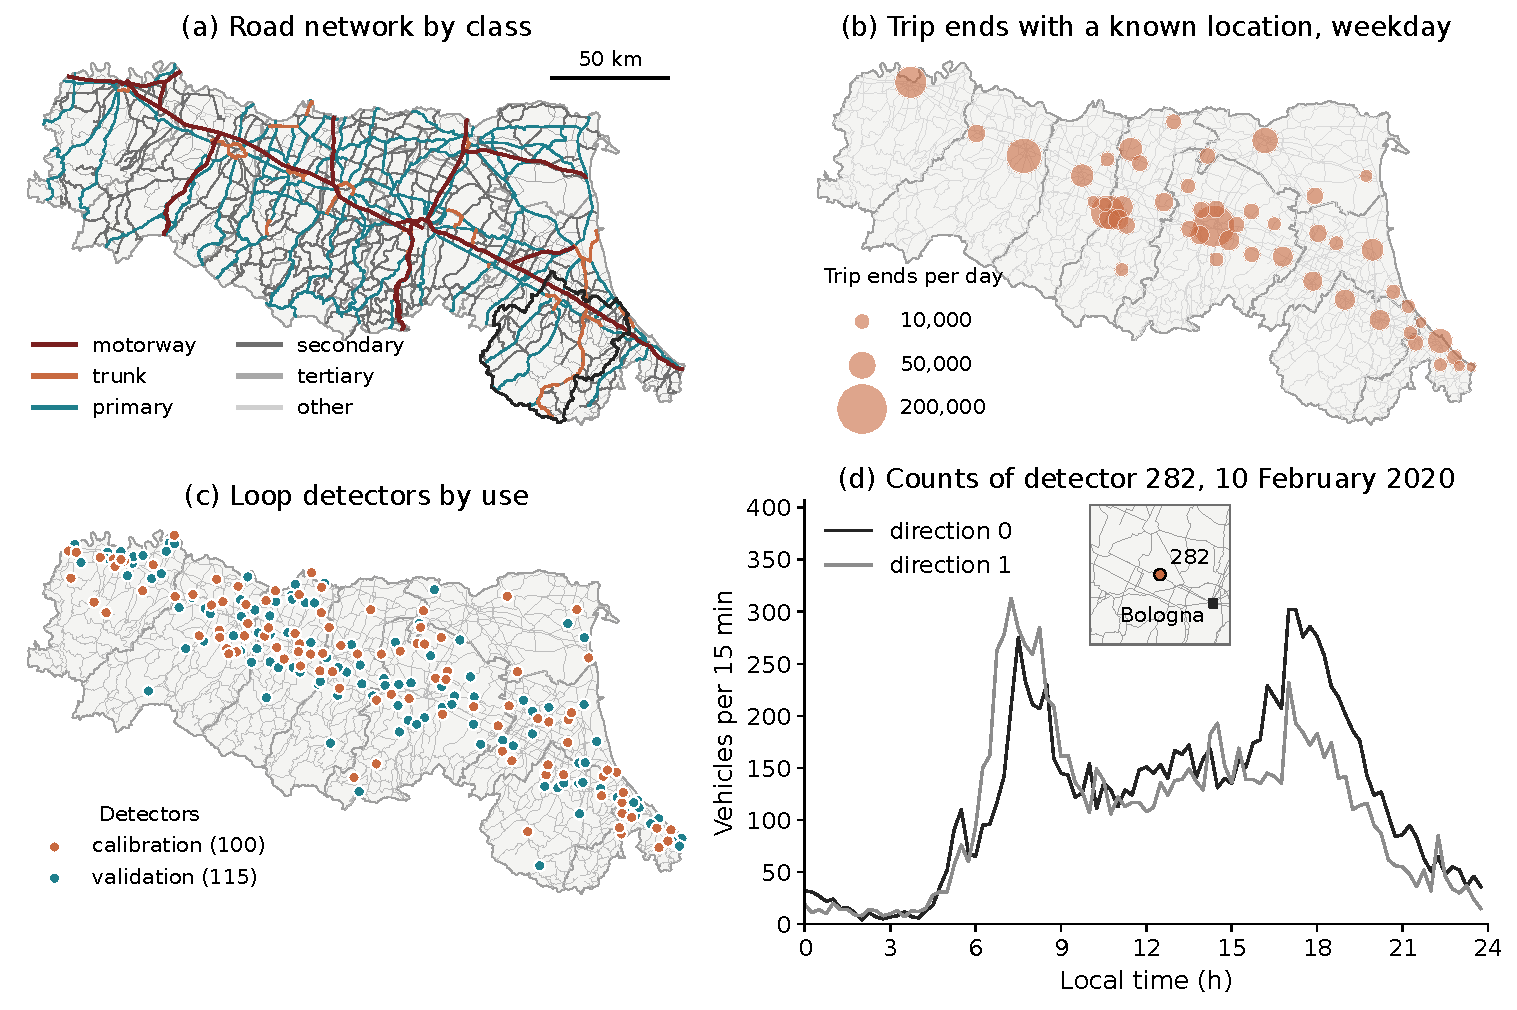
\includegraphics[width=\textwidth]{fig1_inputs.pdf}
\caption{\textbf{Regional domain and observational inputs.} \textbf{(a)} Road network coloured by OpenStreetMap road class; the province of Forl\`i--Cesena, where GPS traces inform route choice, is outlined. \textbf{(b)} Daily trip ends with a known location in the weekday demand, by municipality. \textbf{(c)} Loop detectors of the regional MTS system placed on the network, by their use for daily volumes: the calibration half of February 2020 (100; 60 of them also enter the 2021 tests), validation only (115: the 97 of the test half and 18 used only in 2021), and others (77). \textbf{(d)} Counts of detector 282 near Bologna on 10 February 2020, 15-min resolution, local time. Road network \copyright{} OpenStreetMap contributors.}
\label{fig:inputs}
\end{figure*}

\begin{figure*}[htbp]
\centering
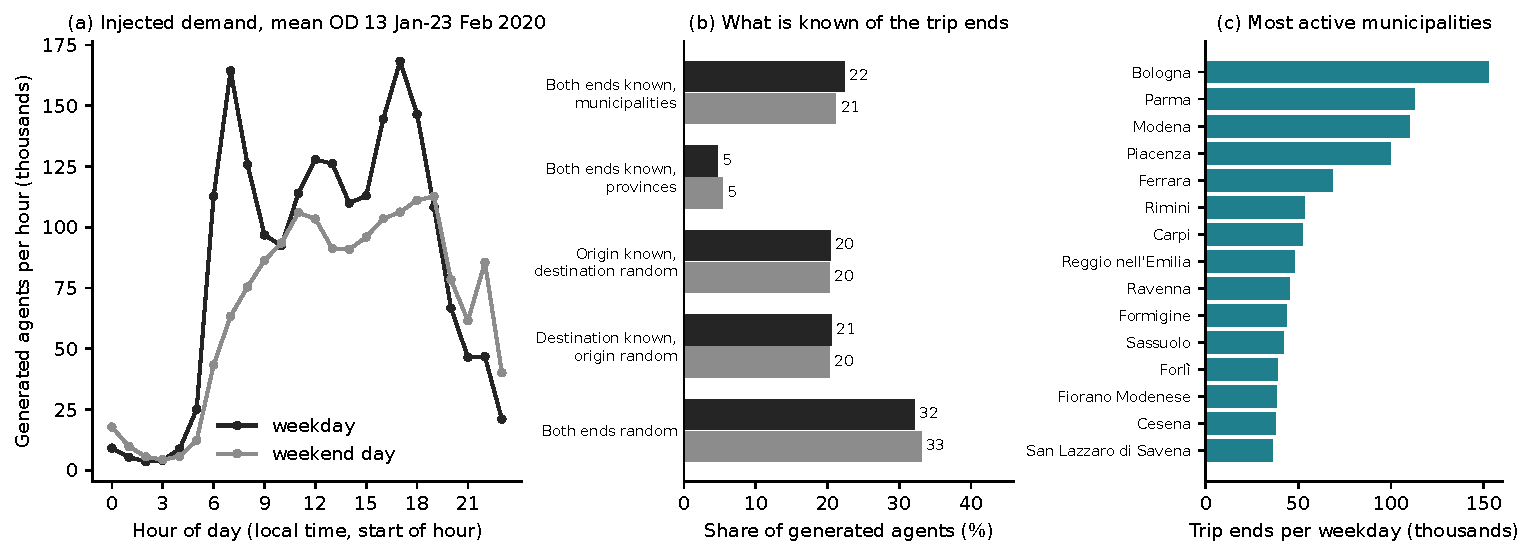
\includegraphics[width=\textwidth]{fig2_demand.pdf}
\caption{\textbf{Simulated demand.} \textbf{(a)} Agents generated per hour for a weekday and a weekend day, after scaling by $k$ and the province factors. \textbf{(b)} Shares of agents by what is known of their trip ends; ``provinces'' are relations with provinces of neighbouring regions. \textbf{(c)} Municipalities with the most trip ends on a weekday.}
\label{fig:demand}
\end{figure*}

The regional MTS system counts vehicles every 15~min in both directions, and 292 of its detectors lie on links of the network (Fig.~\ref{fig:inputs}c,d). For 2020 we use the project archive, and for 2021 the regional open-data release, which reproduces the archive for February 2020. A detector enters the analysis of a given day only if both of its directions are complete. This filter favours busy roads, but relaxing it hardly changes the errors (Supplementary Section~S7).

Viasat provided hourly probe counts per matched link for two campaigns, 10--17 February 2020 (six weekdays and a weekend) and 28 June--4 July 2021 (five weekdays and a weekend), together with the raw traces of private vehicles in the province of Forl\`i--Cesena. About half of the matched links lie in that province (Supplementary Section~S5). Probes played no part in generating or scaling the demand, or in the detector correction.

Phone data were provided as anonymized counts aggregated in space and time, and we accessed no individual records. GPS data were provided as pseudonymized vehicle records and used only to compute link counts, speeds and road-class aggregates. No personal data are reported, and ethics approval was not required.

\section{Methods}
\label{sec:methods}

\subsection{Simulation and route choice}
The \texttt{minimocas} simulator moves agents in steps of 10~s, each at the speed of its link. This speed falls as the density on the link rises, down to a critical speed. Agents with a known origin and destination follow best paths computed with a Dijkstra engine \cite{dijkstra1959} that respects turn restrictions. Agents with a random end instead choose the next link at each node with probability proportional to a transition weight, and travel within a time budget of 5,600~s. For each hour and direction the simulator records how many distinct agents used each link, while virtual counters at the detector locations record crossings. Each run starts empty at midnight, and a given random seed always gives the same run. Traffic is not assigned to an equilibrium \cite{wardrop1952}, and the model does not resolve the congestion phenomena of microscopic traffic-flow models \cite{horni2016,lopez2018,treiber2013}.

To inform route choice, we matched GPS fixes of private vehicles in Forl\`i--Cesena (February 2020) to the road network. For each road class we took the median off-peak speed and the median daily number of probes per link (Supplementary Section~S3), and applied both to all links of that class in the region. The speeds seem stable over time: on the same roads, those of June 2021 have a rank correlation of 0.98 with those of February 2020. The probe numbers set the transition weights of agents with a random end, and they also enter the best-path cost of link $i$,
\begin{equation}
w_i = L_i\left[\alpha + (1-\alpha)\,\frac{1/c_i - 1/c_{\max}}{1/c_{\min} - 1/c_{\max}}\right],
\label{eq:route_cost}
\end{equation}
where $L_i$ is its length, $c_i$ the usage weight of its class and $\alpha=0.5$, so that busier road classes cost less. The simulator also allows a travel-time term, which this variant sets to zero, so that link speed does not enter its cost (Supplementary Section~S3). We chose this variant among shortest-distance, travel-time, mixed and usage-weighted alternatives for its rank correlation between simulated daily volumes and GPS counts in Forl\`i--Cesena; detectors played no role in this selection (Supplementary Section~S3).

\subsection{Demand scaling and local correction}
The OD tables describe one operator's customers, not all traffic, so the number of agents has to be scaled. We multiply it by a factor $k$, which accounts together for coverage, vehicle occupancy and the assumptions on random trip ends, and has no physical meaning of its own. To set it, we split the detectors with complete data in February 2020 into a calibration half (100 detectors) and a test half (97), stratified by province. Weekday observations are averaged and compared with a Monday simulation, and weekend observations with a Saturday simulation. For each day type, $k$ minimizes the mean squared $\log_{10}$(simulated/observed) of daily volumes over a grid from 0.7 to 1.2 (Supplementary Section~S2). Neither the test half nor the 2021 campaign plays any role in this choice.

Throughout the paper, \emph{dispersion} means the standard deviation of $\log_{10}$(simulated/observed) of daily volumes across detectors. It measures how much the error varies from road to road once the overall level is set.

Origins are drawn around the source point, random ends lie within 20~km of the known end, and departures are 45~min earlier than the OD label. The shift is an empirical adjustment with no identified mechanism. These settings were tested on the calibration detectors, and not all of them met the rules fixed for them (Supplementary Section~S2).

Dispersion on the calibration half remained large after the steps above, and a third of its variance lay between provinces (Section~\ref{sec:single_roads}), so we tested one further factor per province. Each trip source with a known location is multiplied by the geometric mean of the factors of its ends inside the region, while sources without a location and ends outside the region keep a factor of one; $k$ is unchanged. The factor of a province starts from one and is multiplied by $10^{-m}$, where $m$ is the median $\log_{10}$(simulated/observed) of its calibration detectors over both day types, and this is done for two rounds. We fixed the adoption rule before the runs: the 95\% paired bootstrap interval of the change in dispersion had to lie below zero on the test half and, only if it did, on the detectors of 2021. The factors add nine parameters, whose values come from the calibration half only.

Detectors also correct the simulation locally. Where a detector exists, we can replace the simulated count with the observed one and spread the difference to nearby roads. Let $u_i(h)$ be the simulated count on the directed link of detector $i$ in hour $h$ and $c_i(h)$ the observed count in that direction; detectors on the same directed link are averaged. The increment at the detector link is
\begin{equation}
\delta_i(h)=\begin{cases} c_i(h)-u_i(h) & \text{if } u_i(h)\ge 1,\\ 0 & \text{otherwise,}\end{cases}
\label{eq:coil_residual}
\end{equation}
so the corrected count $\widetilde u_i(h)=u_i(h)+\delta_i(h)$ equals the observation wherever the simulation has traffic at the detector. From there the increment spreads downstream and upstream. Each adjacent link receives the increment of its parent multiplied by its own simulated share of the flows leaving (downstream) or entering (upstream) the common node, $\delta_{(n_2,n)}=\delta_{(n_1,n_2)}\,u_{(n_2,n)}/\sum_m u_{(n_2,m)}$. The spreading does not enter other detector links, and it stops when the increment falls below one vehicle, after three links along a path, at a forbidden turn or at a closed link. Any negative count is set to zero.

\subsection{How the model is assessed}
\label{sec:validation_methods}
To assess timing, for each GPS-matched link we compare the hourly shares $p_i(h)$ and $q_i(h)$ of the reconstructed and GPS counts over the campaign days, with both directions together, through
\begin{equation}
\mathrm{MAE}_i=\frac{100}{24}\sum_{h=0}^{23}|p_i(h)-q_i(h)|,
\label{eq:profile_error}
\end{equation}
in percentage points (pp). We use three benchmarks, each applied to every link: the OD profile of the demand, the mean profile of the detectors and a flat profile.

We compare daily volumes in both directions at detectors with complete data, using the ratio of total simulated to total observed volume, the Spearman rank correlation, the median absolute $\log_{10}$ ratio and the share of detectors within a factor of two. Intervals come from a paired bootstrap over detectors.

The predictors without simulation take the level from the median volume of other detectors of the same road class and the profile from the mean profile of other detectors. For the test half both are built on the calibration half. For the leave-one-out comparison they are built, like the correction itself, on the other detectors of the same day.

To test the local correction, all detectors of a link are removed from it in turn, and their observations are compared with the corrected reconstruction on that link. The error is $\sum|\widetilde u(h)-c(h)|/\sum c(h)$ over hours, directions and days. We take as depth of the correction the smallest one whose error reduction, in 5-fold cross-validation over the detectors of 2020, lies within one bootstrap standard error of the best depth. Further details are in Supplementary Section~S7.

To measure the value of the OD relations, we ran one simulation per day type without the relations, keeping the number of agents per interval and $k$ but drawing all origins and destinations from population. Since the province factors act through located sources, this simulation loses them too. Under the rule fixed before the runs, the relations are supported if, on the test half of 2020 or on the detectors of 2021, the 95\% interval of the Spearman difference lies above zero or that of the dispersion difference below zero. We added a comparison with GPS link counts after seeing the detector result, and repeated the Monday with three further seeds to measure the variability between runs. We also tried more relations: on the calibration detectors only, we let the relations among the $N$ most active municipalities ($N=100$, 150, 200) keep both ends, retuning $k$ for each $N$. These configurations would have gone on to the 2021 detectors only if they had beaten the model under a rule fixed before the runs (Supplementary Section~S7).

The last tests use only data not used to set the model: the raw simulation on the test half of 2020 and on all detectors of 2021. Each test targets one property, and passing it supports only that property. T1 concerns the level: the volume ratio counts as equivalent to one within 0.80--1.25 if the 90\% bootstrap intervals, over detectors and over provinces, both lie within that margin, as in two one-sided tests. Since the margin is our choice, we also report the smallest one that passes. T2 and T3 concern ranking: T2 asks whether the Spearman correlation exceeds chance, by permuting simulated volumes among detectors, and T3 repeats this permuting only within road class, so that what road class alone explains becomes the null. T4 concerns timing: outside Forl\`i--Cesena, the hourly-share error should be below that of the flat profile (one-sided Wilcoxon signed-rank test). T5 concerns single roads: the share of detector-hours with GEH below 5 should reach 85\%, a criterion of UK guidance for assignment models \cite{tagm31}, where $\mathrm{GEH}=\sqrt{2(m-c)^2/(m+c)}$ for simulated and observed hourly flows $m$ and $c$. P values of T2--T4 are Holm-adjusted over the six tests. We fixed these criteria before computing the outcomes of T3 and T5 and the province intervals, but we had already seen the volume ratios and Spearman correlations. The test half and 2021 had also decided the adoption of the province factors, so for that step these data are not fully untouched.

\section{Results}
\label{sec:results}

\subsection{Level and timing of traffic}
We start with the level of traffic, which is set first. The selected factors are $k=1.0$ on weekdays and $k=0.8$ on weekends. They give a volume ratio on the calibration detectors of 1.00 and 0.98, against 0.90 and 1.10 for the best common factor ($k=0.9$), and the level holds on the test detectors, with a pooled ratio of 0.98. These values are the minima of the grid, although the neighbouring value cannot be told apart from them on the loss alone (Supplementary Fig.~S1). The 20-km radius does not carry over. It reduced dispersion on the calibration detectors from 0.235 to 0.215 (difference $-0.020$ [$-0.033$, $-0.008$]), but on the test detectors, which we used for this comparison once, the difference is $-0.005$ [$-0.016$, $+0.007$].

Province factors then removed most of the regional bias. They range widely: 1.78 for Piacenza, 1.57 for Parma, 1.38 for Ferrara, 1.22 for Modena, 0.97 for Bologna, 0.87 for Forl\`i--Cesena, 0.78 for Ravenna, 0.65 for Rimini and 0.55 for Reggio Emilia. On the calibration half, dispersion falls from 0.215 to 0.187 and the Spearman correlation rises from 0.67 to 0.72. On the test half, dispersion falls from 0.494 to 0.486 (difference interval $[-0.030, -0.0003]$; these values include detector 153, which has no simulated traffic), and in 2021 from 0.409 to 0.397 ($[-0.032, -0.005]$). The rule is thus met in both, though only narrowly on the test half. The Spearman differences, $[-0.01, 0.08]$ and $[-0.01, 0.07]$, include zero. The gain is clearest at the typical detector, where the median absolute $\log_{10}$ ratio, per detector and day type, falls from 0.185 to 0.151 on the test half and from 0.184 to 0.139 in 2021. All later results use this model. On the test half its ratio is 1.01 on weekdays and 0.95 on weekends.

With the level set, we turn to when traffic occurs. Table~\ref{tab:gps_split} separates the links of Forl\`i--Cesena, whose GPS traces also set the route weights, from the rest of the region, which is independent of them. The raw simulation has a median error of 1.16--1.44~pp, well below the flat profile (2.51--2.72~pp) and close to the OD profile of the demand (1.17--1.42~pp). In other words, most of the timing is already in the demand: the simulation does slightly better than the OD profile on weekdays (paired difference $-0.04$ to $-0.08$~pp) and slightly worse on weekends ($+0.04$ to $+0.05$~pp). The mean detector profile beats the raw simulation everywhere (paired difference $+0.07$ to $+0.14$~pp, intervals exclude zero, all days), and it stays ahead after correction, by $+0.06$ and $+0.02$~pp in 2020 and $+0.06$ and $+0.03$~pp in 2021. The correction itself lowers the error by 0.03 and 0.02~pp in 2020, and by 0.00 and 0.01~pp in 2021, and route choice does not change the profiles (Supplementary Section~S3). Pooled over links, the peak hour is 17 for the simulation and 18 for GPS in 2020, and 18 for both in 2021. Because links are spatially correlated, these intervals are optimistic.

\begin{table}[htbp]
\centering
\caption{Median hourly-share error (pp) on GPS links, all days of each campaign. FC: Forl\`i--Cesena, where GPS traces also set the route weights.}
\label{tab:gps_split}
\begin{tabular}{@{}llrrrrrr@{}}
\toprule
Campaign & Area & Links & Raw & Corrected & Mean detector & OD & Flat \\
\midrule
2020 & FC & 442 & 1.16 & 1.09 & 1.03 & 1.17 & 2.72 \\
2020 & Rest of region & 379 & 1.44 & 1.42 & 1.36 & 1.41 & 2.70 \\
2021 & FC & 439 & 1.24 & 1.22 & 1.15 & 1.25 & 2.60 \\
2021 & Rest of region & 379 & 1.39 & 1.36 & 1.30 & 1.42 & 2.51 \\
\bottomrule
\end{tabular}
\end{table}

\begin{figure*}[htbp]
\centering
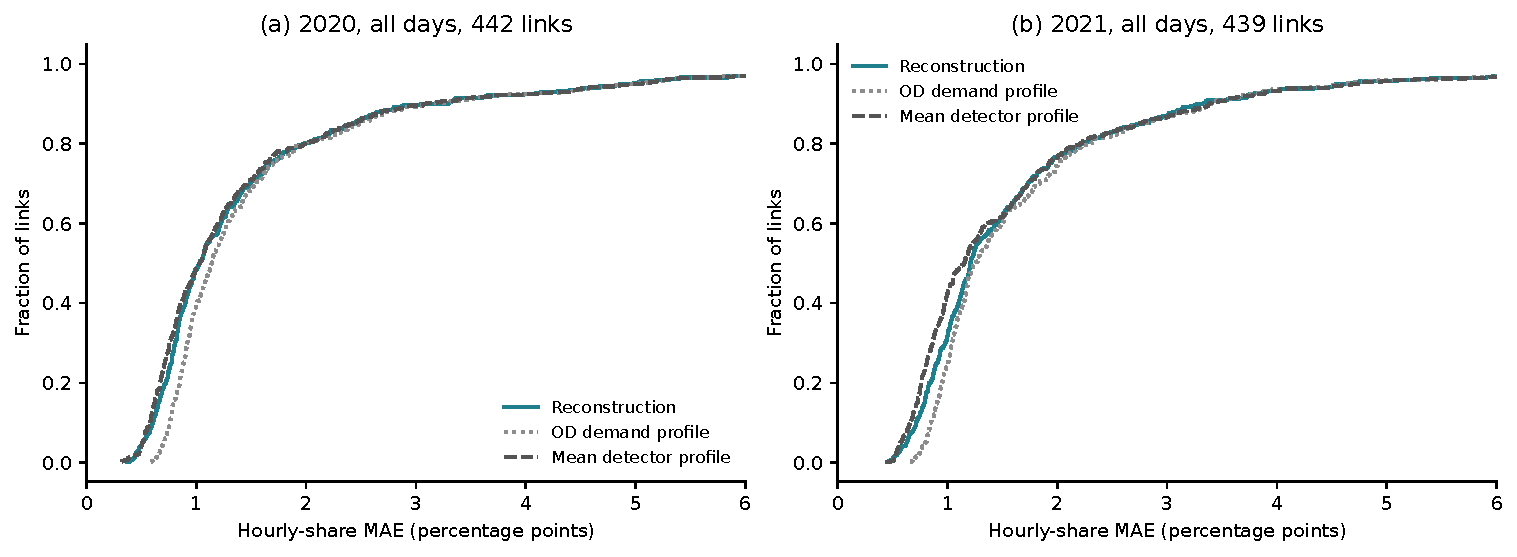
\includegraphics[width=\textwidth]{fig5_validation.pdf}
\caption{\textbf{Hourly shares on all usable matched links.} \textbf{(a,b)} Cumulative distributions of the link error for the reconstruction, the OD demand profile and the mean detector profile. \textbf{(c,d)} Reconstruction and mean detector profile on weekdays and weekends; curves extend beyond the 6~pp limit.}
\label{fig:validation_cdf}
\end{figure*}

Detectors count all vehicles, not a sample, so they give a second view of timing. Figure~\ref{fig:detector_profiles} compares the raw simulation with the four test detectors of lowest error at 15-min resolution. At these detectors the model follows both peaks and the daily level (error 13--15\% on weekdays, 16--21\% on weekends), but they are selected best cases: the median detector has a 15-min error of 35\% and 39\%. Over all test detectors on weekdays (82 detectors), the median correlation of the profiles is 0.96 and the hourly error 39.4\%, with simulated peaks at 8:00 and 17:45 against 7:30 and 17:30 observed. If each detector were given its observed daily level, the error would fall to 14.0\%, so most of the error is a matter of level at the individual road. Weekends (93 detectors) are worse. The median correlation is 0.86, the error 42.8\% and the level-corrected error 22.0\%, and the evening peak falls at 18:45 against 17:30, so the shape is missed as well. These figures use the virtual counters, which are about 8\% below the distinct-agent counts on which $k$ is calibrated, and this contributes to volume ratios of 0.93 and 0.88.

High correlations alone say little, because all detectors share a similar daily pattern. The mean profile of the calibration detectors in fact correlates better with each test detector (median 0.99 on weekdays, difference from the simulation $-0.03$ [$-0.04$, $-0.03$]; 0.98 on weekends, $-0.12$ [$-0.13$, $-0.11$]). With the level of each detector known, this profile gives errors of 7.2\% and 8.2\%, against 14.0\% and 22.0\% for the simulation (Table~\ref{tab:baselines_detectors}). At these detectors, then, the simulation adds no timing information beyond the mean profile.

\begin{figure*}[htbp]
\centering
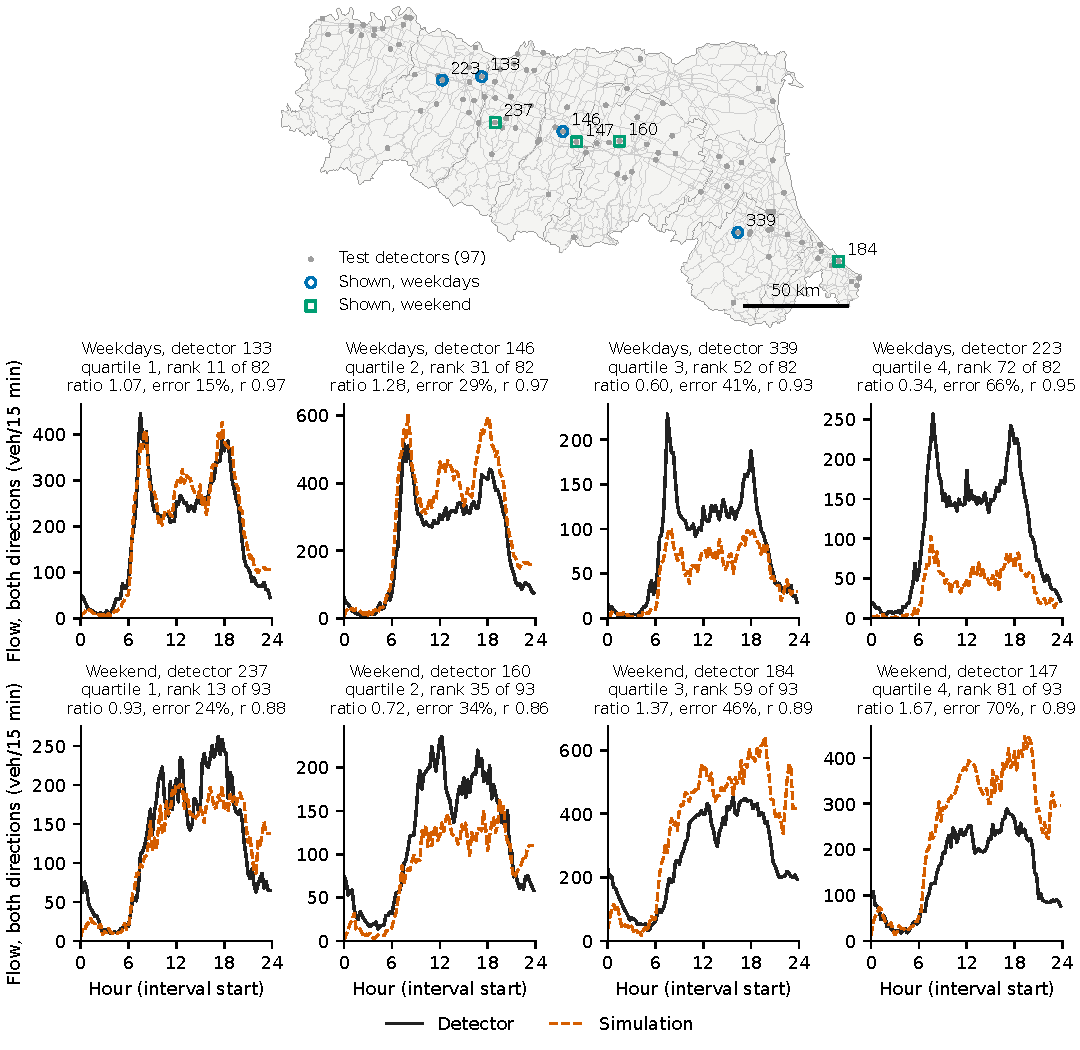
\includegraphics[width=\textwidth]{fig_detector_profiles.pdf}
\caption{\textbf{Best cases at test detectors, 15-min resolution.} The four test detectors with the lowest error, selected for this reason and not representative (distribution in Fig.~\ref{fig:distributions}). Mean observed flow (both directions, February 2020) and raw simulation before any correction, for weekdays (top) and weekends (bottom). Each panel gives the rank among test detectors, the ratio of simulated to observed volume, the 15-min error and the correlation of the profiles.}
\label{fig:detector_profiles}
\end{figure*}

\subsection{Daily volumes and local correction}
Since most of the error at detectors is about level, we now look at daily volumes. On the 97 test detectors of 2020 the volume ratio is 0.97 [0.87, 1.08], the Spearman correlation 0.69 [0.56, 0.79] and the median absolute $\log_{10}$ ratio 0.145 [0.132, 0.197], and 81\% [73, 90] of detectors lie within a factor of two. The 141 detectors of 2021 give similar figures: a ratio of 1.06 [0.98, 1.15], a Spearman correlation of 0.64 [0.52, 0.73], a median absolute $\log_{10}$ ratio of 0.139 [0.115, 0.173] and 84\% [78, 90] within a factor of two. The 2021 agreement is obtained with demand from before the pandemic and a level fixed on winter counts, so it should not be read as a test of demand in that season.

To isolate the effect of route choice, we compare GPS-informed with shortest-distance routing under the same demand, at test detectors outside the province where route choice was set. GPS-informed routing raises the Spearman correlation from 0.61 to 0.71 in 2020 (difference 0.09 [0.02, 0.18]; 87 detectors) and from 0.48 to 0.61 in 2021 (0.13 [0.04, 0.21]; 128 detectors). The median absolute $\log_{10}$ ratio, on the other hand, does not change measurably (0.145 against 0.163 in 2020, difference $-0.02$ [$-0.04$, 0.05]; 0.140 against 0.147 in 2021, $-0.01$ [$-0.05$, 0.04]). Route choice therefore improves the ranking of roads, but not measurably the typical error.

The prediction without simulation (Table~\ref{tab:baselines_detectors}) has a lower median error on daily volumes and more detectors within a factor of two, although the intervals of the differences include zero (weekdays $+0.03$ [$-0.04$, $+0.06$], weekends $+0.02$ [$-0.05$, $+0.04$] in $\log_{10}$ units). Where the simulation does better is in ranking detectors (Spearman 0.66 against 0.41 and 0.67 against 0.48), with intervals that exclude zero ([0.05, 0.45] and [0.01, 0.36]). The hourly errors cannot be told apart ([$-9.6$, $+7.7$] and [$-6.2$, $+9.4$]~pp). Both draw on the calibration detectors: the province factors were set on them, and the predictor is built on them.

\begin{table}[htbp]
\centering
\caption{Raw simulation against a predictor without simulation, test detectors of February 2020. The predictor, built on the calibration detectors, is the median volume of the same road class times the mean profile. Daily volumes and errors come from the virtual counters, both directions.}
\label{tab:baselines_detectors}
\begin{tabular}{@{}lrrrr@{}}
\toprule
 & \multicolumn{2}{c}{Weekdays (82 detectors)} & \multicolumn{2}{c}{Weekends (93 detectors)} \\
Measure & Simulation & Predictor & Simulation & Predictor \\
\midrule
Median $|\log_{10}|$ ratio, daily volume & 0.163 & 0.137 & 0.177 & 0.157 \\
Within a factor of two (\%) & 82 & 89 & 78 & 88 \\
Spearman, daily volume & 0.66 & 0.41 & 0.67 & 0.48 \\
Hourly error (\%) & 39.4 & 40.1 & 42.8 & 41.1 \\
Hourly error with known level (\%) & 14.0 & 7.2 & 22.0 & 8.2 \\
Median profile correlation & 0.96 & 0.99 & 0.86 & 0.98 \\
\bottomrule
\end{tabular}
\end{table}

All results so far describe the raw simulation. We now add the local correction. When each detector is withheld in turn at depth 3, the error falls from 41.3\% to 37.7\% in 2020 (reduction 3.7~pp [1.9, 5.7]; 152 detectors) and from 44.1\% to 39.7\% in 2021 (4.4~pp [2.1, 7.0]; 141 detectors). The correction thus removes about one tenth of the error at detectors it has not seen. The 2020 set includes the calibration detectors and the depth was selected on 2020 only, so 2021 is the independent estimate (Supplementary Section~S4). The median detector goes from 38.0\% to 33.3\% and from 39.1\% to 36.7\%; 66\% and 62\% of detectors improve, 19\% and 23\% worsen, and the Spearman correlation of the volumes rises from 0.70 to 0.71 and from 0.64 to 0.67. The reduction is similar on weekdays and weekends (2020: 3.9 and 3.2~pp; 2021: 4.4 and 4.5~pp), though on different sets of detectors. Cross-validation over 2020 gives 0.7, 1.9, 3.3, 3.6, 3.9 and 4.0~pp at depths 1 to 6. The best depth is the edge of the grid, and the one-standard-error rule selects depth 3. The correction cannot help a detector with no simulated traffic: detector 153 stays at zero.

On the same records, the predictor built on the other detectors of the same day gives 36.9\% in 2020 and 37.6\% in 2021. The raw simulation is above it, with an interval of the difference that includes zero in 2020 ($[-1.5, +10.0]$~pp) and barely excludes it in 2021 ($[+0.1, +13.7]$~pp). The corrected reconstruction cannot be told apart from it ($[-4.8, +6.1]$ and $[-4.0, +8.4]$~pp), with central estimates slightly in favour of the predictor, and only 48\% and 49\% of detectors are better predicted by the correction. At single sections, therefore, the simulation has not been shown to predict better than road class and the other detectors. Detectors also differ widely (Fig.~\ref{fig:distributions}): half of them have a corrected error between 23\% and 50\% in 2020 and between 25\% and 53\% in 2021, and the simulation tends to underestimate trunk roads, although few detectors lie in that class.

\begin{figure*}[htbp]
\centering
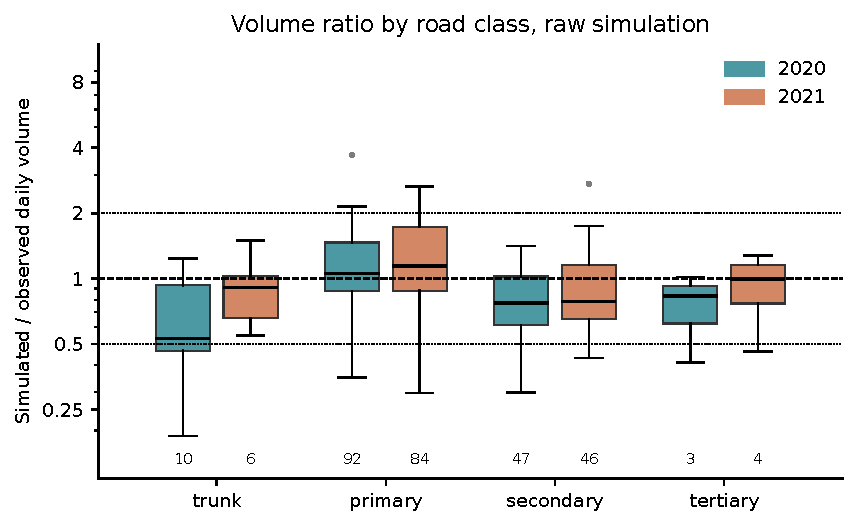
\includegraphics[width=\textwidth]{fig8_distributions.pdf}
\caption{\textbf{Agreement over all detectors.} \textbf{(a)} Hourly error at withheld detectors, raw simulation and corrected reconstruction. \textbf{(b)} Ratio of simulated to observed daily volume by road class, raw simulation, with the number of detectors below each box; dashed line: equality; dotted lines: factor of two. One detector with zero simulated traffic is not shown in (b). Boxes: quartiles and median; whiskers: 1.5 interquartile ranges.}
\label{fig:distributions}
\end{figure*}

With the correction we can draw the full traffic field. Figure~\ref{fig:simulation} shows the reconstruction with all detectors used, together with the best case of the leave-one-out test on 10 February 2020. Detector 258 recorded 24,230 vehicles that day, and when it is withheld the reconstruction on its link gives 25,504 (error 9\%, hourly correlation 0.99). This is what the model can achieve where it works best, and it is not typical: detector 258 has the lowest directional error of the 61 detectors complete that day, while the median is 32\%, as the distribution in Fig.~\ref{fig:distributions} also shows.

\begin{figure*}[htbp]
\centering
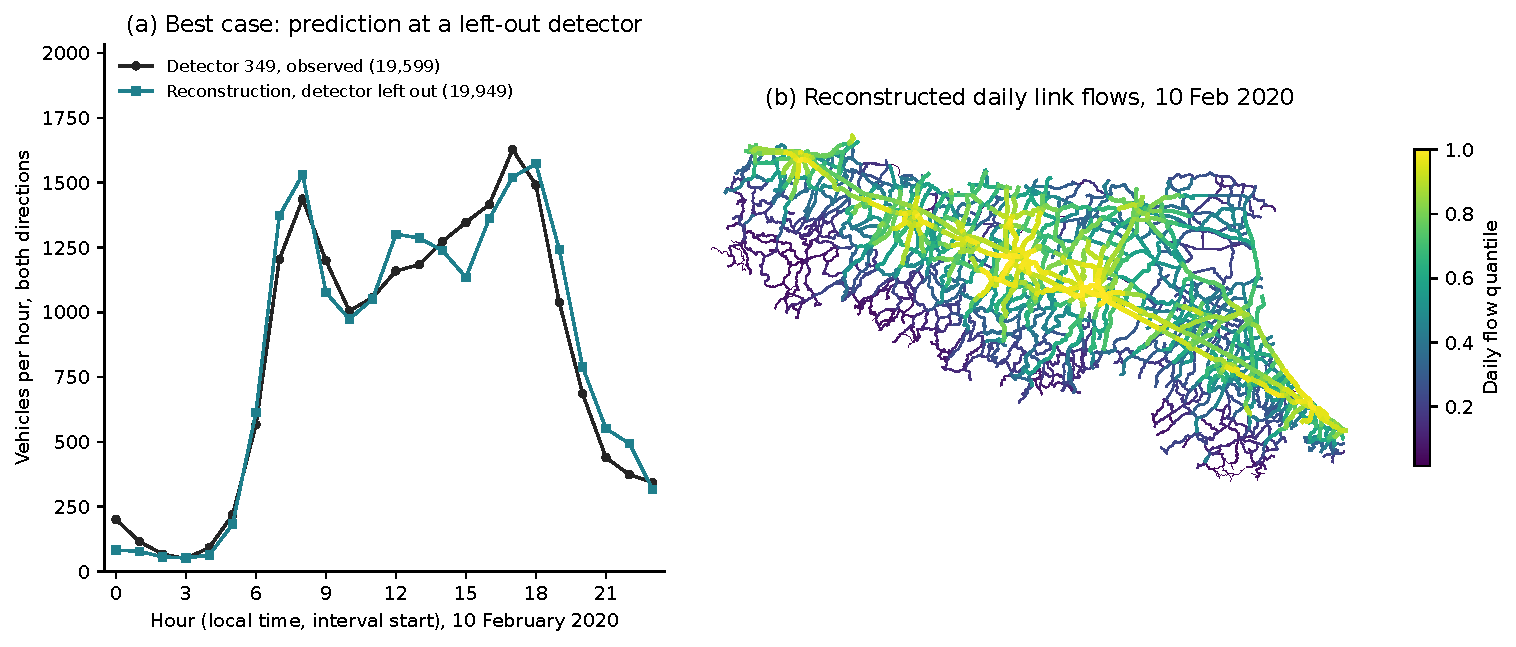
\includegraphics[width=\textwidth]{fig3_reconstruction.pdf}
\caption{\textbf{Reconstructed traffic field.} \textbf{(a)} Best case among the 61 detectors complete on 10 February 2020: hourly counts of detector 258 (both directions) and the reconstruction on its link when that detector is withheld from the correction and all others are used; totals in parentheses. \textbf{(b)} Reconstructed daily link flows, coloured and scaled by flow quantile. Basemap \copyright{} OpenStreetMap contributors \copyright{} CARTO.}
\label{fig:simulation}
\end{figure*}

\subsection{Value of the OD relations}
\label{sec:od_relations}
We now ask what the OD relations themselves add, which is the least clear case. The rule is met in one of four comparisons, the Monday on the test half (Spearman difference 0.07 [0.01, 0.14]). The other three have intervals that include zero (Saturday 0.05 [$-0.00$, 0.11]; 2021, 0.06 [$-0.03$, 0.16] and 0.03 [$-0.02$, 0.09]), and no dispersion difference excludes zero. We do not read this as support for the relations, because the comparison does not isolate them: the simulation without relations also loses the province factors, which were set on detectors, and the four comparisons are not adjusted for multiplicity. Rank correlation with GPS link counts is also unchanged, both in Forl\`i--Cesena (0.68--0.73 with relations, 0.68--0.74 without) and elsewhere (0.48--0.65 and 0.47--0.66), with all intervals including zero. Chance between runs does not account for these differences: between seeds on the Monday, the Spearman correlation ranges over 0.001 and the volume ratio over 0.003, and the median coefficient of variation of a detector's daily volume is 0.9\%.

Extending the relations to more municipalities did not meet its rule on the calibration detectors and was not adopted, and the model barely captures the direction of travel (both tests in Supplementary Section~S7).

\subsection{Error at single roads}
\label{sec:single_roads}
The results so far leave a large error at single roads, so we look at what kind of error it is. It is not noise. The day-to-day deviation of a detector's count from its own mean has a median of 0.017 in $\log_{10}$ units, against a dispersion of 0.172 on the Monday and 0.200 on the Saturday of the calibration half. Nor does the error of a detector change much between day types (correlation 0.96, 78 detectors) or between winter 2020 and summer 2021 (0.98, 110 detectors). Without the province factors, province explains 32\% of its variance on the Monday, road class 9\% and observed volume 5\% (43\% together), and detectors less than 5~km apart have correlated errors (0.56, 20 pairs). With the factors, province explains 6\%, road class 10\% and volume 7\% (23\% together), and the correlation between nearby detectors is no longer distinguishable from zero (0.11 below 5~km, $-0.06$ at 10--20~km).

Misplaced detectors do not explain this. Comparing detector coordinates with the OpenStreetMap geometry, we flagged 5 of 292 as doubtful (two on closed links, one 870~m from its link, two on a road with a different reference). The median distance from the link is 8~m, and on the 193 evaluated detectors not flagged, dispersion remains 0.247 (without province factors, all days). What remains is a stable property of each road that neither regional level, road class nor volume captures. It may reflect the way the model represents local access and the roads missing from the regional network, together with a choice of route that depends on road class only, but we have not tested this.

\subsection{Formal tests and contribution of each source}
\label{sec:tests}
Finally, we test each property on independent data (Table~\ref{tab:tests}). The ranking of roads exceeds chance in both campaigns, even when road class is held fixed (adjusted $p<0.001$), and on links outside the calibration province the simulation beats the flat profile in timing on 97--98\% of links ($p<10^{-60}$). The level is equivalent to observation within 0.80--1.25 in both campaigns, whether detectors or provinces are resampled, and the smallest margin passing in both is about 1.19. The province interval needs some caution. It rests on few provinces, and each of them received its own factor, so on the calibration half it is favourable by design, and on the other data it is only partly independent. Criterion T5 fails clearly, with about one third of detector-hours having GEH below 5 against the target of 85\%. A regression across detectors points the same way. The slope of $\log_{10}$ simulated on $\log_{10}$ observed volume is compatible with one in 2020 and just below it in 2021, but $R^2$ is only 0.19 and 0.16, in line with the large error at single roads.

\begin{table}[htbp]
\centering
\caption{Final tests on data not used to set the model values, raw simulation. Intervals for T1 are 90\%; for T5 and the slope, 95\%. FC: Forl\`i--Cesena.}
\label{tab:tests}
\begin{tabular}{@{}p{5.8cm}p{4.4cm}p{4.4cm}@{}}
\toprule
Test & Test half, 2020 (97 detectors) & 2021 (141 detectors) \\
\midrule
T1 Volume ratio, resampling detectors & 0.97 [0.88, 1.06]: pass & 1.06 [0.99, 1.13]: pass \\
T1 Volume ratio, resampling provinces & [0.84, 1.10]: pass & [0.95, 1.15]: pass \\
T2 Spearman above chance & 0.69, $p<0.001$ & 0.64, $p<0.001$ \\
T3 Spearman within road class & $p<0.001$ & $p<0.001$ \\
T4 Timing against flat, outside FC (error, pp) & 1.44 against 2.70, $p<10^{-60}$ & 1.39 against 2.51, $p<10^{-60}$ \\
T5 Detector-hours with GEH $<5$ (target 85\%) & 34\% [30, 38]: not met & 33\% [29, 36]: not met \\
Slope, log--log volumes ($R^2$) & 0.94 [0.74, 1.17] (0.19) & 0.82 [0.66, 1.00] (0.16) \\
\bottomrule
\end{tabular}
\end{table}

Table~\ref{tab:sources} answers the question of this paper by collecting the effect of each source on data not used to set it. Phone data give the timing and, with detector scaling, the level; GPS improves the ranking of roads; detectors also bring a small local gain through the correction. The OD relations are the one input whose value we could not show.

\begin{table}[htbp]
\centering
\caption{What each source adds, on data not used to set it. Differences are in the sense of adding the source; negative errors are improvements. Intervals are 95\% bootstrap.}
\label{tab:sources}
\begin{tabular}{@{}p{3.5cm}p{5.2cm}p{5.8cm}@{}}
\toprule
Source & Role & Effect \\
\midrule
Mobile-phone OD, total and timing & agents per interval & hourly-share error 1.1--1.4~pp against 2.5--2.7 flat; not better than the mean detector profile \\
Mobile-phone OD, relations as used (20\% of activity between municipalities) & known trip ends & Spearman $+0.03$ to $+0.07$, interval excludes zero in one of four comparisons; not separable from the province factors (see text) \\
Detectors, half & scale $k$ by day type & test ratio 0.97; 1.06 in 2021 \\
Detectors, half (nine values) & province factors & median $|\log_{10}|$ ratio per detector and day type 0.185 to 0.151 on the test half, 0.184 to 0.139 in 2021; dispersion $-0.008$ and $-0.012$ (intervals exclude zero) \\
GPS traces & route weights & Spearman $+0.09$ [0.02, 0.18] and $+0.13$ [0.04, 0.21] outside the province; median error not measurably different; profiles unchanged \\
Detectors, all & local correction & hourly error $-3.7$~pp [$-5.7$, $-1.9$] and $-4.4$~pp [$-7.0$, $-2.1$] at withheld detectors; profile error $0.00$ to $-0.03$~pp on GPS links \\
\bottomrule
\end{tabular}
\end{table}

\section{Discussion}
\label{sec:discussion}
We asked what each data source contributes to a regional traffic model. With eleven demand-level parameters (two by day type, nine by province), the model reaches the observed overall level and timing, and each source has an identifiable role. Three results limit what it can claim. First, the timing comes from the daily profile of the demand, and at the links tested that profile adds nothing beyond the mean profile of the detectors. Second, the correction removes about one tenth of the error at withheld detectors and has little effect on hourly profiles, especially in 2021. Third, the OD relations used by the model have no clear effect of their own on road volumes. The province factors do improve the typical road by correcting a regional bias, but they are empirical. A factor of 1.78 or 0.55 cannot be read as a difference in phone coverage or car use without further evidence, and the factors would have to be re-estimated for another period or region.

The third result concerns the model as built, not the information in the tables. Most traffic is already drawn at random, relations are placed at one point per municipality, and the network and the route weights may largely decide which roads carry traffic. Detectors and GPS also test road volumes rather than relations between places, so the OD may be correct where it is not tested. In the same way, a value of $k=1$ cannot be read as the inverse of the operator's coverage, because it depends on what the tables represent and on the assumptions on random trip ends.

At the detectors, the reconstruction is no more accurate than a predictor without simulation, although the simulation ranks the test half better. That predictor, however, offers no routes, no consistency across the network and no response to changes in demand, and detectors are not a random sample of roads. We did not test these properties of the simulation here.

Among the limitations, the largest remaining error is the level at individual roads, which neither the timing, the province factors nor the correction removes. Our validation data were not entirely untouched: the test half and 2021 decided the adoption of the province factors, and the gain on the test half met the rule only narrowly. Several settings were chosen on the calibration half without a demonstrated gain on the test half: the 20-km radius is not confirmed, the origin spreading did not meet its rule, and the 45-min shift has no identified mechanism. The model does not reproduce the weekend shape or the hourly differences between directions. Since the model uses one fixed random seed, differences between configurations do not include the variability between runs, which we measured only on the Monday. The factor $k=0.8$ was chosen on Saturday and also applied to Sunday. The correction spreads increments within the same hour, without travel time. Finally, the simulation starts empty at midnight, and 122 links remain closed although at least one of them, or the detector placed on it, is inconsistent with the counts.

\section{Conclusions}
\label{sec:conclusions}
We have presented a regional mobility model that combines mobile-phone demand, detector counts and GPS, and measured what each adds on data not used to set it. Rescaling by day type and province gives the observed overall volume on independent detectors and removes most of the regional bias, GPS-based routing improves the ranking of roads outside its province, and the local correction reduces the error at withheld detectors. The overall timing comes from the daily profile of the demand. The OD relations that the model uses, 20\% of the activity between municipalities, have no clear effect of their own on road volumes. Formal tests on independent data support the overall level, the ranking of roads and the timing, but not accuracy at single roads. There the error is stable and specific to each road, the model does not outperform predictors based on road class and other detectors in hourly error, and it falls well short of the usual GEH criterion. A regional simulation of this type should therefore be justified by its consistent network-wide picture and by its ability to represent changes in demand, which still have to be tested, rather than by its accuracy at instrumented sections.

\section*{Supplementary information}
Additional file 1 describes the data layers and the demand classes (S1), the demand scale and the changes tested on the calibration detectors (S2), the simulation model and the route-choice variants (S3), the detector correction and its sensitivity to depth (S4), additional validation results (S5), the reproduction of all results (S6) and further details of data and methods (S7).

\section*{Abbreviations}
GEH, Geoffrey E. Havers statistic; GPS, Global Positioning System; MAE, mean absolute error; MTS, regional traffic monitoring system of Emilia-Romagna; OD, origin--destination; pp, percentage points.

\section*{Declarations}

\subsection*{Availability of data and materials}
The mobile-phone OD tables (TIM) and the Viasat GPS data are proprietary and were used under agreements that do not allow redistribution; requests for access should be addressed to the data providers. MTS loop-detector counts are published by Regione Emilia-Romagna under a CC BY licence (open-data catalogue, dataset ``Sistema MTS -- Flussi di traffico al quarto d'ora''). Road classes are derived from OpenStreetMap (\copyright{} OpenStreetMap contributors, ODbL). The road graph, the aggregate results behind every figure and table, and the link-level validation metrics without probe counts are included in the code repository. The simulation configurations derive from the mobile-phone OD tables and are not distributed. The simulator \texttt{minimocas}, the detector correction and all analysis scripts are available at \url{https://github.com/federicobellisardi/multi-sensor-traffic-reconstruction}. Supplementary Section~S6 outlines the steps that reproduce the results.

\subsection*{Competing interests}
C.M. and A.F. are employed by Mindicity, which contributed to the development of the modelling framework. The other authors declare no competing interests.

\subsection*{Funding}
F.B. received support from the Italian National Operational Programme on Research and Innovation 2014--2020 (CCI 2014IT16M2OP005), FSE REACT-EU, Actions IV.4 and IV.5.

\subsection*{Authors' contributions}
F.B. designed the study, developed the reconstruction and validation pipeline, performed the analyses and wrote the manuscript. C.M. and A.F. contributed to the simulation framework and to the processing of the mobile-phone and detector data. A.B. conceived the modelling approach and supervised the study. All authors read and approved the final manuscript.

\subsection*{Acknowledgements}
We thank TIM (Telecom Italia) for the mobile-phone data, Viasat for the GPS data, the Mobility and Viability Section of the Emilia-Romagna Region for the MTS detector data, and Stefano Grandi, Claudio Domenichini and Elena Grossi for discussions.

\bibliographystyle{sn-basic}
\bibliography{references}
\end{document}
